\documentclass[a4paper,11pt]{article}

\usepackage[margin=1in]{geometry}

\usepackage{graphicx}
\usepackage{amsfonts}
\usepackage{tabularx}
\usepackage{amsmath}
\usepackage{amsthm}
\usepackage{thmtools}
\usepackage{booktabs}
\usepackage{color}
\usepackage{xspace}

\usepackage{tablefootnote}

\definecolor{cnblue}{RGB}{14,73,137}

\usepackage[utf8]{inputenc}

% Setup style to mimic our GoogleDocs style
\usepackage[sfdefault,lining]{FiraSans} %% option 'sfdefault' activates Fira Sans as the default text font
%\usepackage[fakebold]{firamath-otf}
\usepackage[mathrm=sym]{unicode-math}
\setmathfont{Fira Math}
\usepackage[T1]{fontenc}
\renewcommand*\oldstylenums[1]{{\firaoldstyle #1}}


% Setup headers to be similar
\usepackage{titlesec}
\titleformat*{\section}{\fontsize{14pt}{21pt}\selectfont\bfseries\color{cnblue}}
\titleformat*{\subsection}{\fontsize{14pt}{21pt}\selectfont\color{cnblue}}
\titleformat*{\subsubsection}{\fontsize{13pt}{20pt}\selectfont\itshape\color{cnblue}}
\renewcommand{\paragraph}[1]{\textbf{#1.}}
\setcounter{secnumdepth}{2}

\newcommand{\parait}[1]{\noindent\textit{#1}}

\usepackage{setspace}
\setstretch{1.15}

\usepackage[parfill]{parskip}

\usepackage{enumitem}
\setlist{noitemsep}


\usepackage{hyperref} 
\usepackage{cleveref}

\newcommand{\code}[1]{\textsf{#1}\xspace}

\newcommand{\notificationkey}{\code{notification\_key}}
\newcommand{\defaulttime}{\code{default\_time\_in\_venue}}
\newcommand{\arrivaltime}{\code{arrival\_time}}
\newcommand{\departuretime}{\code{departure\_time}}

\newcommand{\locationname}{\code{name}}
\newcommand{\locationlocation}{\code{location}}
\newcommand{\salt}{\code{salt}}

\newcommand{\qrbase}[1]{\ensuremath{\code{QR}_{\code{#1}}}\xspace}
\newcommand{\qrentry}{\qrbase{entry}}
\newcommand{\qrexit}{\qrbase{exit}}
\newcommand{\qrtrace}{\qrbase{trace}}
\newcommand{\qrcode}{\code{QRCode}}

\newcommand{\group}{G}
\newcommand{\generator}{g}
\newcommand{\grouporder}{p}
\newcommand{\pk}{pk}
\newcommand{\pkH}{\pk_{H}}
\newcommand{\sk}{sk}
\newcommand{\skH}{\sk_{H}}
\newcommand{\hash}{H}

\newcommand{\ctxtmsg}{c_{\textsf{msg}}}
\newcommand{\entryprime}{\textsf{entry}'}
\newcommand{\exitprime}{\textsf{exit}'}

\newcommand{\enc}{\textsf{Enc}}

\begin{document}

\begin{center}
  \color{cnblue}
  \fontsize{18pt}{27pt}\selectfont
  % Title
  {\bf\textsf{CrowdNotifier}}\\
  % Subtitle
  \fontsize{15pt}{22pt}\selectfont
  Decentralized privacy-preserving presence tracing\\
  % Version
  \fontsize{11pt}{18pt}\selectfont
  \textit{Version 8 October 2020}\\[11pt]
  % Authors
  \fontsize{12pt}{18pt}\selectfont
  \textit{Wouter Lueks (EPFL), Seda Gürses (TU Delft), Michael Veale
    (UCL), Edouard Bugnion (EPFL), Marcel Salathé (EPFL), Carmela Troncoso
    (EPFL)}\\[11pt]
  % Contact note
  \fontsize{11pt}{15pt}\selectfont
  \textit{Contact the first author for the latest version}\\[12pt]
\end{center}

% TODO: remove for camera-ready, but force page numbers for now
% Force page numbering
\thispagestyle{plain}
\pagestyle{plain}

\section*{Executive Summary}
We are publishing this document to inform the discussion revolving around the design and implementation of presence tracing systems and to present our version, CrowdNotifier. We welcome feedback on the requirements and properties of presence tracing systems we identity as well as the design we propose, so that missing requirements and protections can be identified and the overall system can be improved.

Contract tracing aims to slow down the spread of viruses (e.g., SARS-CoV-2) by identifying close contacts of persons that have been infected with the virus. Traditionally this is a manual effort where contact tracers interview SARS-CoV-2-positive people to determine who their close contacts are. Digital proximity tracing aims to augment this effort by rapidly notifying contacts that have been in close proximity to an infected person, even if the infected person could themselves not identify that contact.

To account for airborne transmission in spaces with bad ventilation or physical but non-prolonged contacts, epidemiologists have pointed out the need to also consider people that have been sharing a semi-public location with a SARS-CoV-2-positive person for a prolonged time as contacts to be notified. Such locations include restaurants, bars, classrooms, and places of worship; but also events such as concerts and meetings. 

Contact tracing systems, therefore, need means to notify these ``presence contacts'', i.e., people present a such locations. Digital proximity tracing, such as Exposure Notification, does not provide such means, as its operation means that only people at the venue who were in close physical proximity to the SARS-CoV-2-positive person would be notified.

Existing systems to enable presence tracing typically require a user to “check-in” to a location, such as using a hand-written or electronic form, or using a sensor on a device, such as a camera to scan a QR code. 

In this document we present a simple presence tracing system, CrowdNotifier,
that is \emph{easy to use}, can be used to \emph{effectively notify} any presence contacts of SARS-CoV-2-positive persons, while at the same time providing \emph{strong privacy and abuse-prevention properties}.
\section{Motivation}

Epidemiological studies have recently pointed to the potential of airborne
transmission beyond the close physical contact distance of 1--2 meters
\cite{prather2020airborne}. While the overall contribution of this transmission
route remains unknown, multiple studies have shown that clusters -- i.e., events
with a comparatively high number of transmission events -- play a crucial role
in the epidemiological dynamics of the COVID-19 pandemic
\cite{adam2020clustering, wong2020evidence}.

Such clusters seem to predominantly occur in crowded indoor environments with limited ventilation. Such environments may include restaurants, bars, classrooms, and places of worship as well as events such as concerts, meetings, and private reunions. For quarantine considerations, contact tracers are thus increasingly including not only individuals who were in close proximity to an infected person, but also those who were present at the same location. 

These places and events can host a considerable amount of people, and notifying
them thus increases the load of contact tracers. When this load is already high due to the amount of positive cases, manual notification associated to presence can become a bottleneck. Digital presence tracing solutions aim at reducing the load of contact tracers in two dimensions: supporting contact tracers in deciding who to notify, and facilitating the notification process. 

The deployment of digital presence solutions requires the creation of infrastructure that inevitably generates new data. The potential misuse of this data raises unease in the population and put at risk the wide adoption of these technologies which in turn reduces their utility as support for contact tracing.

For these reasons, it is important to design digital presence tracing in a privacy-preserving manner, anticipating the dangers associated with mass deployment, to facilitate adoption. In this work, we take into account the following four factors:

\paragraph{Checks on power and population control}
Digital presence tracing systems facilitate the notification of individuals who meet epidemiologically-defined criteria (e.g., were present at a location within a certain time window compared to a potential index case). Deployed presence tracing systems do so at the sole discretion of a central authority such as a public health agency. Such infrastructure can, however, be easily abused if a central authority utilises it for non-epidemiological purposes: With a registry of locations, and background knowledge (e.g., about the demographics or characteristics of visitors to those locations), segments of the population can be ordered to quarantine with no additional infrastructure or cost.

This contrasts with proximity tracing technologies such as Exposure Notification, where to trigger notifications with this effect would require the deployment of infrastructure (e.g., Bluetooth emitters, or coopted smartphone applications~\cite{DehayeR20}) which could not operate with the same certainty, costless scalability, or undetectability. When combined with legal obligations to quarantine and/or individuals' personal desire not to infect others, systems of presence tracing that operate at the discretion of a central authority could serve as a method of population control. It could, for example, be used as a tool for voter suppression, particularly as political actors often already hold detailed background knowledge as to the location and demographics of voters holding different electoral intentions. As a consequence, digital presence tracking systems should be designed to effectively meet genuine epidemiological goals while introducing safeguards against this potential abuse of power by central authorities.

\paragraph{Safeguards for user privacy}
A second group of concerns around presence tracing relates to issues of individual privacy. Systems which leak individuals’ location histories can be abused in a variety of ways depending on to whom the leak occurs. Leaks to central authorities may result in persecution; leaks to other users, such as perpetrators of intimate partner violence and abuse, may exacerbate coercive control~\cite{ChatterjeeDOHPF18,FreedPMLRD18,LevyS20}. Digital presence tracing systems should be designed to remove or minimise these risks.

\paragraph{Concerns for the confidentiality of locations}
A third group of concerns relates to the confidentiality of locations, and societal harms that can result from rendering the existence of social gatherings, meetings and communities centrally legible and machine-readable. While many venues already volunteer or are legally compelled to be part of large and often publicly accessible databases (e.g., bars for licensing or mapping purposes), this is not the case for all epidemiologically relevant gatherings. For some, such as political or religious gatherings, a technology that demands they formally register their existence to an entity outside their community (such as a central authority) may itself pose a threat regardless of the individual privacy protections or safeguards on the power to issue notifications\footnote{See e.g., in the United Kingdom, The Health Protection (Coronavirus, Collection of Contact Details etc and Related Requirements) Regulations 2020 schedules 1--4.}. While technological safeguards may help mitigate some concerns, at the heart of this issue is the definition (which may be in law) of what constitutes a relevant `location' for epidemiological purposes. Choosing to broaden this beyond existing, self-published locations (e.g., most restaurants, bars, cafés) will be a political choice that cannot be easily specified or limited by a technological protocol, and the breadth of the definition should be considered in the proportionality of introducing any presence tracing system. Therefore, to ensure that the protection provided by the system is independent of policy decisions, we aim to build a solution that does not rely on such a registry of locations.

Additionally, the system should aim to maintain confidentiality of which locations were visited by SARS-CoV-2-positive people to prevent stigmatization and shaming of owners or organisers, and visitors.

\paragraph{Gracious dismantling}
A final concern relates to the sunset of the system. Because the system is introduced in a situation of emergency, it is important to ensure that, after this situation ends, the impact of the system is minimal. Ideally, control on the sunset should be on the users' side, without creating a dependency on authorities. Successful sunset of the system should not rely on authorities dismantling infrastructure (e.g., by stopping servers, or deleting databases).

Moreover, it is desirable that once the system is not necessary anymore, authorities dismantle all infrastructure supporting the system. In other words, none of the infrastructure created to support the system should prevail after system operation stops.

\section{Entities and Terminology}

In this white paper we use the following terminology for the entities in a presence-tracing system. All presence tracing systems we examine, whether digital or analog, use the following high-level entities or a subset thereof:

\begin{description}[topsep=2pt, partopsep=2pt]
\item[Visitor] somebody who visits a location. Sometimes called user. There can be many visitors.
\item[Location] a semi-public location (for example, bar, restaurant, religious building, events venue, or meeting place) or an event which takes place in one or more locations (for example, an exhibition). There can be many locations.
\item[Location Owner] the owner or manager of a location. For simplicity, we assume each location has one owner. An owner may manage many locations.
\item[Health Authority] the public health-authority that determines which visitors of which locations to notify. Usually, there is only one health authority.
\item[Backend] a backend server that can (potentially) interact with visitors, locations, and the health authority. Usually there is only one backend.
\end{description}

Presence tracing concerns crowds that gather at a certain location at a certain time. This could be a crowd on a Friday evening at a bar, or on a Tuesday afternoon meeting in a community center. For readability we use the term ``location'' to refer to locations at a specific time as well as specific events (that may happen within one or more physical locations).

Health authorities may use different criteria to determine when to notify visitors to a location for a given time slot  (e.g., visitors were wearing masks, there were barriers or large separation between groups). We use the following terminology to indicate locations whose visitors should be notified and the respective visitors:
\begin{description}[topsep=2pt, partopsep=0pt]
\item[Trace location] a location that was visited by one or more SARS-CoV-2-positive persons, and whose visitors should be notified.
\item[Presence contact] a person that was present at a location around the same time as one or more SARS-CoV-2-positive persons and should thus be notified.
\end{description}

\section{Overview of CrowdNotifier}

We present CrowdNotifier. CrowdNotifier aims to help health authorities to implement presence tracing while being easy to use for users and being easy to deploy for venue owners and event organizers. Moreover, the system aims to be respectful of the following design principles, already implemented in decentralized contact tracing:

\begin{itemize}
\item \textit{Privacy by design}: no private/sensitive data should be stored in any central database. Moreover, private data should not be derivable from data (e.g., logs) that are stored for operational purposes.
\item \textit{Purpose limitation by design}: abusing the system for population control, location tracing, or other objectives other than sending notifications should be difficult if not impossible.
\item \textit{Voluntary basis}: Use of the digital system is not mandatory. A non-digital fallback must always be available.
\end{itemize}

We design the system under the following assumptions:

\begin{enumerate}
\item The health authorities has the means to identify which locations have been visited by a SARS-CoV-2-positive person, and at what times those visits happened.
\item The digital system can rely on the use of a mobile app on the user’s device. This app can be either separate or integrated with existing proximity tracing solutions. In either case, the system must be designed such that the privacy properties of both proximity and presence tracing  are guaranteed. The design proposed later on in this document fulfills this property.
\item Presence tracing should be possible even if the SARS-CoV-2-positive person did not themselves use the app.
\item Users can be trusted to follow notifications from the app, just like they would when they are notified of a close contact by a digital contact tracing app.
\end{enumerate}

The first assumption implies that CrowdNotifier does not need to provide means to identify which locations had a prolonged visit of a SARS-CoV-2-positive person. Just the means to notify other visitors that this even happened and they are at risk and need to take precautions.

The second assumption delimits the technological capabilities on which the design can rely: the kind of sensors that can be used, and the connectivity and the computational capabilities that can be expected.
The use of an app guarantees that the system can notify all visitors, even in the case in which the SARS-CoV-2-positive person did not themselves use the app. 

The third assumption supports the voluntary nature of the system. It is in line with the current approach used in many places, which assumes that visitors can put their actual phone numbers and name in an attendance log that can be provided to the authorities. There is empirical evidence that many fake numbers are used. In fact, one can reasonably expect better compliance from a privacy-preserving digital solution (where citizens should take action when actually exposed) vs. the classic solutions (where citizens should take action -- i.e, write down their real phone number -- when attending the venue).

The fourth assumption implies that there is no need to design an enforcement mechanism to ensure that notified users that receive a notification comply with the instructions they receive.

\subsection{A walkthrough of the system}
The following example illustrates the operation of the CrowdNotifier system. For illustration, we use a venue as location (e.g., an association’s meeting place, a mosque, a church, a meeting room, a bar, a restaurant, a night club), but we recall that a location could also represent an event that spans different locations (e.g., a demonstration). 

In \name users store encrypted records for each visit on their phone. These
records can only be decrypted using the decryption key for the corresponding
time slot. Without this key, these records reveal nothing, guaranteeing users'
privacy against strong attackers. To initiate tracing, the health authority -- together with the location owner -- computes and publishes the proper time-slot specific decryption keys. Apps regularly download these keys and use them to try to unlock the encrypted records. If encryption succeeds, the user may need to be notified.

To build this time-slot specific encryption system, \name uses an identity-based encryption (IBE) scheme. Each location owner acts as the trusted authority. In this setting, users store records of visits by encrypting against a time-based identity for the location they visit. The location owner with the health authority compute the corresponding identity-based decryption keys to enable tracing.

\paragraph{Setting up}
Suppose Charlie manages a location for which she decides to use \name presence notification to help her visitors break transmission chains after an outbreak. To do so, Charlie first uses \name to generate and print two QR codes: an \emph{entry code} and a \emph{tracing code}. The entry code contains information describing the venue as well as an identity-based master public key. The tracing code contains the corresponding master private key.

Charlie posts the entry code in a place where visitors can scan it (e.g., at the entrance, or on the tables), and keeps the tracing code private. See Figure~\ref{fig:overview}, Setup.

\paragraph{Visiting the location}
When entering the location, visitors can use the app or not. If they do, they scan the QR code posted at the entry to the location. The app shows the name of the location and asks the user to confirm the check in.
See Figure~\ref{fig:overview}, Entering a venue. If they do not use the app, they write their contact information on an attendee list.\footnote{The collection of non-digital data should also be made according to the data minimization principle. It suffices to provide contact information. For the purpose of notifying visitors, these visitors do not need to be identified.}

Once the app learns the departure time (e.g., because the user explicitly checks out after a reminder from the app), the phone stores a private record containing the identity-based encryption (using the location's master public key) of the entry and departure times, using the entry hour as part of the identity.
Our choice of identity-based encryption scheme ensures that these ciphertexts do not reveal the location for which they were created to anyone with access to the user's phone as long as the location owner does not compute and reveal the specific decryption key.


\begin{figure}
  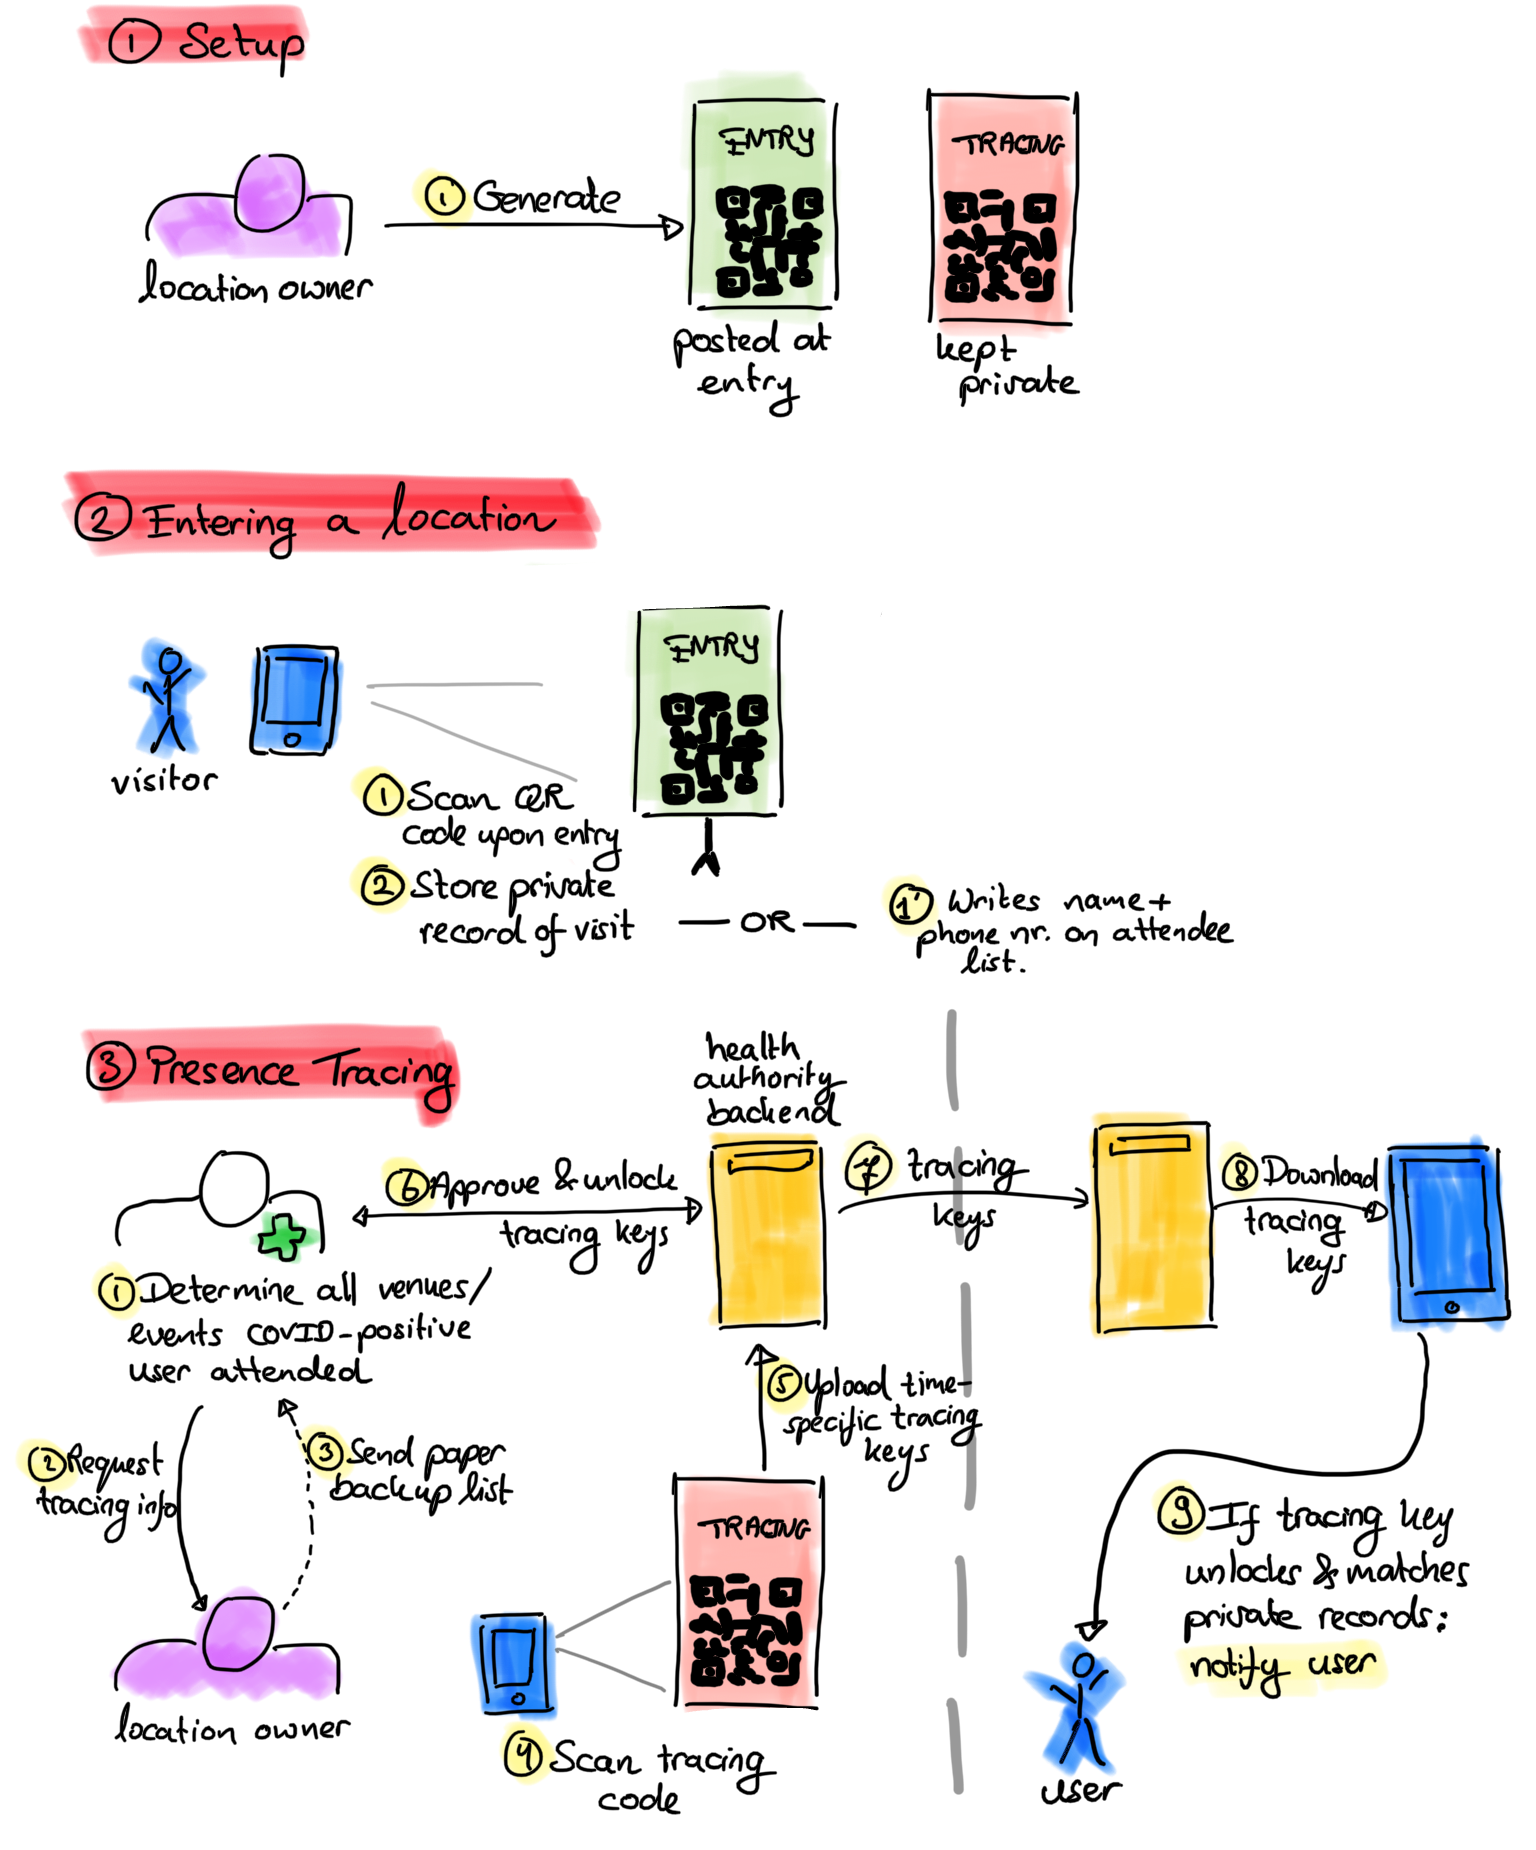
\includegraphics[width=\textwidth]{figures/overview2}
  \caption{\label{fig:overview}Overview of the core operations in our proposal for Presence Tracing}
\end{figure}

\paragraph{Presence tracing}
First, health officials need to determine which locations the SARS-CoV-2-positive person attended (step 1, Figure~\ref{fig:overview}, Presence Tracing), e.g., using the traditional interviewing process in which different positive users report having been at a location. The health official then contacts the owner for each of these locations, requesting two things (step 2):

\begin{itemize}[topsep=0pt, partopsep=0pt]
\item The paper backup list (step 3)
\item That the location owner uploads tracing keys, i.e., identity-based decryption keys, for the affected time interval (steps 4 and 5).
\end{itemize}

The health official checks and approves the uploaded tracing keys (step 6). This ensures that the data corresponds to the requested location. Then, the health authority’s backend makes available the tracing keys (steps 7 and 8) to all users of the system. 

Phones download the provided tracing keys to try and unlock (i.e., decrypt) private records stored on the phone. If unlocking succeeds, it means that the user was at a location with a SARS-CoV-2-positive person. In this case, the phone recovers the user's entry and departure times for the venue. The phone then determines if there is an epidemiologically relevant overlap between the user’s time at the location and that of the SARS-CoV-2-positive person. If there is, the phone notifies the user (step 9).

\section{Requirements and properties}

The following is a preliminary list of requirements. This list might be incomplete. Also, the security and privacy requirements make some assumptions on the infrastructure. They are not necessarily complete wrt specific designs that use other infrastructure.

\subsection{Functional requirements}
Following the principles of data-minimization, we require that presence contacts are notified. However, as with proximity tracing, this does not necessarily mean that any party learns the identity or contact information of presence contacts.

\paragraph{F1: Paper fallback option available} The system should support a paper-based fallback option for people that do not have, or do not want to use the smartphone application. 

\paragraph{F2: Presence contacts are notified} After a positive SARS-CoV-2 diagnosis for a person, all presence contacts should be notified. Since the SARS-CoV-2-positive user might have used the fallback, notification should be possible even if the SARS-CoV-2-positive user did not use the app (see F1).

\parait{Challenge:} Capturing exact arrival and departure time might conflict with usability (NF1). While informing the app of arrival should not be complicated, it seems more difficult to require another user action upon departure of a location. Automating departure measurements would seem to require access to sensors that conflict with NF2. Alternatively, the app can ask that users estimate for how long they are planning to stay at a location, or the app simply estimates the departure time (e.g., 2h after arrival or closing time).

\paragraph{F3: Non-presence contacts are not notified} After a positive SARS-CoV-2 diagnosis for a person, any visitors to a location that do not have an epidemiologically relevant overlap with visits of the SARS-CoV-2-positive person are not notified.

\parait{Challenge:} The need for this requirement depends on judgements made by local health authorities (e.g., taking into account the local situation, the need to be convervative/proactive, and the latest epidemiological insights).

\parait{Challenge:} this property might be difficult to achieve, depending on how accurate time-keeping is and how accurate SARS-CoV-2-positive visitors (or their devices) can recall their visiting times. The default can be closing time. The app can also poll the user later, asking for the (approximate) departure time of the user. Or the app can ask the user only once it determines a potential overlap with a SARS-CoV-2-positive person.

\subsection{Non-functional requirements}
\paragraph{NF1: Ease of use for users} To ensure adoption, the system should be easy to use from a user’s perspective. And in particular no more complicated than base-line paper-based solutions.

This requirement implies that when users have to scan QR codes, these should be small enough (in terms of the amount of data that they contain) that they can be reliably printed/displayed and then scanned by users’ devices.

\paragraph{NF2: Easy deployment for locations} To ensure adoption of the system in a large number of locations, the system should not require (special) hardware at locations or server infrastructure managed by locations. 

\paragraph{NF3: Speed of notification} After the SARS-CoV-2-positive user has completed the required steps --- for example, they informed the contact tracing team of which locations they visited --- any presence contacts should receive a notification quickly.

\parait{Challenge:} background tasks of apps do not necessarily run frequently.
While ``entering'' a location might bring the app to the foreground, and thus cause the OS to assign more background-time; this is not necessarily enough to pick up events days later from background tasks. It might be better therefore to integrate with existing proximity tracing apps.

\paragraph{NF4: Small bandwidth and computation requirements} The system should have a small bandwidth and computation requirement on the side of the user.

\subsection{Security/Privacy requirements}

\subsubsection{Privacy of users}

\paragraph{PU1: No central collection of personal data} The presence-tracing system should not require the central collection of personal data (e.g., name, IP-address, e-mail address, telephone number, locations visited) of people that visit a location. Nor should the system be able to infer location or co-location data of either visitors or notified visitors.

For the purpose of presence tracing, the health authority is allowed to learn which locations a SARS-CoV-2-positive person visited. 

\parait{Corollary:} this requirement also implies that any central infrastructure used to facilitate the system (e.g., a server) should not be able to deduce that a specific IP address visits a specific location. 

\paragraph{PU2: No collection of personal data at a location} The system should not require collecting at the location itself personal data (e.g., name, e-mail address, telephone number) of people that visited that location. The sole exception to this is the paper-based fall-back approach.

\paragraph{PU3: No location confirmation attacks given phone} The system should hide which locations somebody has visited. PU1 and PU2 imply that this information should not be available centrally or at the location itself. This information should not be available to attackers that have access to the phone. In particular:
\begin{itemize}
 \item The UI should not reveal which locations the user visited (e.g., to prevent (retroactive) location tracking by intimate partners and law enforcement).
 \item The data stored on the phone should not reveal or enable confirmation of visited locations to determined attackers (e.g., law enforcement). Such attackers can gain access to internal storage (i.e., information stored internally by the app), and can also be assumed to have visited specific locations.
\end{itemize}
 
\parait{Inherent limitation of decentralized systems.} In decentralized systems, the phone locally determines if the user should be notified. Therefore, such systems cannot prevent location confirmation attacks with trace locations.

\paragraph{PU4: Do not leak notifications through network traffic} The network traffic (if any) should not reveal that a specific user has been notified.

\paragraph{PU5: Do not leak SARS-CoV-2-positive status through network traffic} The network traffic (if any) should not reveal that a specific user has received a positive test result.

\subsubsection{Confidentiality of locations}
\paragraph{PL1: Hide which locations had a SARS-CoV-2-positive case from non-visitors} Attackers that never visited a location, should not be able to determine whether that location had a SARS-CoV-2-positive case.

\paragraph{PL2: Hide which locations had a SARS-CoV-2-positive case from non-contemporal visitors} An attacker that visited a location, but not during the time when a SARS-CoV-2-positive person was present, should not be able to determine whether that location had a SARS-CoV-2-positive case.

\parait{Challenge:} this requirement is more tricky than PL1, as it requires that there is information that is only available to visitors around a specific time. This then implies active displays (or at least changing QR codes) to achieve.

\parait{Inherent limitation:} No functional presence tracing system can hide that a location is positive from contemporal visitors of that location. This would be in direct violation of the core functional requirement that presence contacts are notified (F1).

\paragraph{PL3: No new central database of locations/events} The system does not create (or rely on) a central database capturing information about all locations. This avoids creating a new database with events (e.g., political and religious gatherings) for the purpose of presence tracing.

\parait{Corollary:} this requirement also implies that organizers and owners should be able to produce the QR codes anonymously (e.g., using the Tor browser). 

\subsubsection{Security}

\paragraph{S1: No fake notifications (targeting of users)} The system should make it impossible to target specific individuals, thereby causing them to be quarantined

\paragraph{S2: No population control (targeting of locations)} The system should make it impossible to target sensitive locations (gay bar, biker hangout, bars/places-of-worship in specific neighbourhoods, etc.), thereby causing all the visitors to be quarantined.

\parait{Inherent limitation.} If an infected person deliberately visits sensitive locations, the functional requirements imply that visitors of this location must be notified. So, at best, we can protect against people that did not visit a location.

\parait{Confused deputies:} Because of requirement (F1), the system must accept locations self-reported by SARS-CoV-2-positive users. Therefore, a malicious SARS-CoV-2-positive user might use the system as a confused deputy to mark a location as a trace location, triggering notifications.

The extent of this problem depends on when the health authorities mark a location as a trace location (e.g., does this require several reports) and whether health authorities can verify that the SARS-CoV-2-positive person was at the claimed location.

\paragraph{S3: Automatic dismantling of the system}
The dismantling of the system should not depend on central authorities to take action, e.g., to delete keys or data. Instead, as soon as users and location owners stop using the system, any remaining infrastructure should be automatically rendered useless.

\section{Design}
The proposed system consists of two parts: (1) a fall-back paper solution and (2) a digital solution using a smartphone application that scans QR codes. The existence of the fallback solution ensures compliance with F1. Both parts are decentralized, but the digital solution achieves better privacy properties.

\subsection{Design choices}
We made several design choices for the digital system to satisfy the above requirements.

\parait{Optional action upon departure.} For the sake of useability (NF1) and robustness, the system will still function if users do not (or forget to) perform an action when leaving a venue. Instead, the system will use an estimate for the time people usually spend at this venue as default.

\parait{(Semi-)Static QR codes for venues.} To ensure easy deployment for locations (NF2), venues and events can use static QR codes. As a result of this choice, PL2 becomes impossible to achieve. Users that visited a location at any time, can later confirm that this location was marked as a trace location; even if the user was not there on the same day/time.

If protecting against this attack is essential, venues and organizers can instead generate new QR codes for every day or time-slot (for example, displaying them on screens). Requiring the user to have been present to determine whether the location is notified. Which is the best any system can do.

\parait{Single-purpose: notify presence contacts.} The app does not retain a list of visited locations to aid contact tracers in their interview with a SARS-CoV-2-positive user. Instead — as is currently the norm — contact tracers must rely on interviews with the SARS-CoV-2-positive person to determine which locations that person visited, when and for how long.

The system also does not facilitate contacting or identifying the owner of a location (e.g., a venue owner, or event organizer). Instead — as is currently the norm — contact tracers should rely on public records and information provided by the SARS-CoV-2-positive user to get in touch with the location owner.

The single purpose of the system is to notify presence contacts.

\parait{No network connections required when entering a location/event.} All necessary information is embedded in the QR code. This ensures the system works even when there is no Internet connection. Moreover, the system does not generate any observable network traffic when entering locations as a result.

\parait{Regular polling by phones rather than push messages.} The use of push notification services such as Firebase requires that users enroll with and connect to 3rd party services. This is not necessary for our use case.

\subsubsection{Non goals}

\parait{Verification of attendance.} The system does not aim to provide contact tracers with a proof that a user has been at a location. As a result, users might lie about where they have been, potentially violating S2.

\parait{Enforcing quarantines.} The system does not aim at providing authorities with the ability to enforce quarantine after notification. We assume that notified users will follow instructions from the health authorities with respect to the actions they should take.

\subsubsection{Why not just use the GAEN framework?}
Doesn’t the GAEN framework already offer precisely what is needed to do this type of colocation tracing?
 
No — to use the GAEN framework, locations must operate infrastructure (violating NF2). In particular, locations must operate one or more Bluetooth beacons that transmit RPIs as in the GAEN framework. (And, modifications are necessary to ensure that any mobile device inside the location will detect the transmitted RPIs as “close”, and to mitigate individuals not inside the location (e.g. in a flat upstairs, or a neighbouring establishment, from too easily registering these modified signals.)

\subsection{A fallback solution: pen \& paper}
To satisfy the requirement for a paper-based fallback solution for visitors that do not have or want to use the app (F1), we present a fallback pen \& paper solution. This solution also serves as a baseline for the proposed digital solution.

This approach works as follows:

\begin{enumerate}
\item A location keeps a box/list per day or time-slot.
\item Every visitor enters contact information (e.g., name and phone number) into the box/list.
\item Only when contact tracing reveals that a SARS-CoV-2-positive person visited a location during a specific time: the authorities receive the corresponding list \& contact every presence contact on this list.
\item After 14 days, the boxes/lists are destroyed.
\end{enumerate}

Pros/cons:
\begin{itemize}
\item[+] No central list of information about who visited which location (PU1)
\item[+] Easy to use for users (NF1)
\item[+] Easy to use/deploy for locations (NF2)
\item[+] Fast notification and no bandwidth requirements (NF3 \& NF4)
\item[+] No privacy reductions through network traffic (there is none) (PU4 \& PU5)
\item[+] No information on phone that can be exploited (PU3)
\item[+] Population control requires cooperation of owners/organisers and health authorities (S2)
\item[+] Automatic dismantling (S3)
\item[-] Personal data is available locally at the locations (PU2)
\item[-] ``System''/contact-tracers learn locations of presence contacts (PU1)
\item[-] ``System''/contact-tracers can target individuals (S1)
\end{itemize}

\subsection{Digital presence tracing}



The digital presence tracing solution works as follows. We assume that users have the corresponding app installed on their phone.

\paragraph{Setup} The health authority generates a public-private encryption key pair $\pkH, \skH$; a cyclic group $\group$ of prime order $\grouporder$ with generator $\generator$; and a public hash function $\hash$.

\paragraph{QR Code Generation} A location takes as input the name and location (e.g., address) of the event, and generates a set of QR codes as follows:
It picks a random value salt and derives a private key $\sk$ by committing to the name and location by computing
\begin{equation*}
	\sk = \hash( \locationname \parallel \locationlocation \parallel \salt ).
\end{equation*}

It computes the corresponding public key $\pk = \generator^{\sk}$ and it picks a random symmetric key \notificationkey.
It constructs three QR codes:
  \begin{align*}
    \qrentry &= \qrcode(\textsf{``entry''} \parallel \pk \parallel \notificationkey \parallel \defaulttime) \\
    \qrexit &= \qrcode(\textsf{``exit''} \parallel \pk ) \\
    \qrtrace &= \qrcode(  \enc(\pkH, \locationname \parallel \locationlocation \parallel \salt \parallel \notificationkey)  )
  \end{align*}
and prints them. The codes \qrentry and \qrexit are pasted at the entrance(s) of the venue. The code \qrtrace is kept private by the organizer.

The private key $\sk$ is needed to perform any type of presence tracing. The data needed to recompute it are stored in an encrypted form in \qrtrace. Cooperation of the health authority is needed to decrypt these values.

The notification key \notificationkey is used to encode messages by the health authority so that they can only be decrypted by apps of users that actually visited the corresponding location. This protection is not perfect. Anybody that knows or learns \notificationkey can subsequently make it public.

The commitment trick used to compute the private key $\sk$ ensures that the private key is bound to the name and location of the venue, enabling the health authority to verify that they publish the correct key after decrypting \qrtrace.

\parait{Safely generating the QR codes.} It is essential that the salt is only known to the venue owner. Therefore, these QR codes cannot be generated server-side. We propose to use client-side JavaScript to statelessly generate PDFs containing the QR codes. This PDF should contain three pages:
\begin{itemize}
\item A page that includes the entry QR code \qrentry, with clear instructions labeling this as the entry code, explanations of fall backs, and the name of the location.
\item A page that includes the entry QR code \qrexit, with clear instructions.
\item A page with the tracing QR code \qrtrace.
\end{itemize}

The QR code should encode a URL that opens the app directly, without generating further network traffic.

\paragraph{Entering/leaving a venue} Upon entering a venue, the user uses their app to scan the corresponding entry QR code. Let $\pk$ be the public key in the QR code and \defaulttime the default time we assume people stay at the venue. The app:
\begin{enumerate}
\item Picks a random value $r \mod \grouporder$.
\item Computes 
  \begin{equation}
    (\generator^r, \pk^r, \enc(\pk, \arrivaltime \parallel \notificationkey \parallel \defaulttime))
  \end{equation}
\end{enumerate}
and stores this tuple together with a label for the current day.

Optionally, upon leaving the venue users can scan the exit QR code, the app behaves as before, but then stores $\enc(\pk, \departuretime \parallel \textsf{``departure''})$ as ciphertext instead.

These steps compute a Diffie-Hellman key exchange between the user’s device, holding private key $r$ and public key $\generator^r$ and the venue’s public key $\pk$. The resulting shared key is $\pk^r$. The user’s device only stores the public key $g^r$ and the shared key $\pk^r$.

The stored tuples are constructed in such a way that they hide which venue the user visited to everybody that does not know the private key $\sk$ corresponding to the public key $\pk$ of the venue. (Assuming the DDH assumption holds in $\group$.)

Devices automatically delete any entry older than 10 days.

\paragraph{Initiating contact tracing}
After the contact tracing team of the local health authority has determined that a SARS-CoV-2-positive person has visited a location during the contagious period, they proceed as follows. Let entry+ and exit+ the times that the SARS-CoV-2-positive person entered and exited this location.
\begin{enumerate}
\item The contact tracing team creates a case number to manage locations related to this patient.
\item They then contact the owner/organiser of the location and request upload of the data in \qrtrace to the health authority’s server using the given case code. To do so, the owner/organizer scans the QR code with their app, enters the case code, and approves the data upload to the health authority’s server.
\item The health authority’s server decrypts the uploaded data to recover name, location, salt and \notificationkey.
\item The contact tracing team checks that all uploaded information from the tracing codes (in particular, the name and location) corresponds to the locations the SARS-CoV-2-positive person visited. They remove any extra uploads under this case code.
\item For each approved upload $\locationname \parallel \locationlocation \parallel \salt \parallel \notificationkey$, the health backend server recomputes $\sk$ as above. It encrypts a message $\ctxtmsg$ to the user using $\notificationkey$ and publishes the recomputed $\sk$ together with the corresponding entry and exit times and $\ctxtmsg$.
\item Finally, the owner/organizer generates new QR codes as per Setup above and removes the old codes from the venue.
\end{enumerate}

The check performed in step 4 and the subsequent recomputation of $\sk$ in step 5 ensures that a malicious or coerced venue owner cannot substitute the QR code of another location without this being detectable by the health authority.

\paragraph{Presence tracing and notification.}
The user’s app regularly (say, every few hours) performs the following checks:
\begin{enumerate}
\item The app downloads all $(\sk, \entryprime, \exitprime, \ctxtmsg)$ tuples that were published since the last time it checked.
\item For each $(\sk, \entryprime, \exitprime, \ctxtmsg)$ tuple downloaded, the app proceeds as follows.
  \begin{enumerate}
    \item It finds all matching entry records for the day corresponding to entry+ and exit+. That is, for every stored tuple $(h, k, c)$ (corresponding to the values $(\generator^r, \pk^r, c)$ stored earlier); the app selects records where $h^\sk$ matches $k$.
    \item For all matching records, the app decrypts the ciphertext $c$ using $\sk$ to recover corresponding entry/exit times, default times in the venue, and the \notificationkey.
    \item The app uses these times (using the default time if no departure time is recorded) to determine if the user’s presence at the venue overlaps with the time the SARS-CoV-2-positive user was at the venue. If there is overlap, the app decrypts $\ctxtmsg$ using the recovered key \notificationkey and notifies the user by displaying this message.
  \end{enumerate}
\end{enumerate}
  
\subsubsection{Functionality analysis}
\parait{F1.} See above. Using paper-based fallback solution.

\parait{F2 \& F3.} The digital system keeps track of accurate entry times. Therefore, everybody that potentially overlaps with the SARS-CoV-2-positive user at a location can be notified. Satisfying F2. Moreover, if users scan exit codes (or if default duration of a visit is representative) users will not be notified if they did not overlap with SARS-CoV-2-positive user. Largely satisfying F3.

\parait{NF1.} Users only need to scan a QR code upon entry (and optionally departure) of a location. No other actions are required.

\parait{NF2.} Locations do not require additional infrastructure.

\parait{NF3.} Presence contacts are notified within hours of contact tracers obtaining the required information from the location owner/organizer.

\parait{NF4.} The bandwidth costs are very small. Less than 256 bytes per location that is marked as a trace location (depending on the length of the supplied message).

\subsubsection{Security and privacy analysis}

\parait{PU1 \& PU2.} There is no central collection of private data related to users. There is also no data collection at the venue (apart from the fallback method). Therefore PU1 \& PU2 are satisfied.

\parait{PU3.} Provided that the venue owner (or event organiser) and the health authority do not collude, location confirmation attacks against data stored on the phone are not possible as long as a location is not marked as a trace location.

As argued above, the sk corresponding to a venue is needed to confirm a location. This value is held in encrypted form by the venue owner, and can only be decrypted by the health authority. Therefore, an attacker needs to coerce (or collude with) both the venue owner and the health authority and gain access to a user’s phone to perform a confirmation attack.

\parait{PU4 \& PU5.} The system does not generate any sensitive network traffic. All phones download information from the backend server. None of them ever send any information.

\parait{PL1.} To confirm that a location is a trace location, the adversary needs to know the corresponding public key pk. This value is on the QR code at the entrance to the venue. Since non-visitors do not know this value, PL1 is normally satisfied. However, malicious visitors can publish the association between pk and a location to enable confirmation attacks.

\parait{PL2.} PL2 is not satisfied, unless the venue owner generates new QR codes for every day or time-slot.

\parait{PL3.} PL3 is satisfied. The system does not generate nor rely on the creation of any central database related to venue owners or event organisers.

\parait{S1.} Individual users cannot be targeted. Any published tracing information will always target all visitors to a specific location.

\parait{S2.} To target a location requires (1) having access to the private key sk corresponding to that location and (2) convincing the health authority to publish it.

The private key sk key is only available by decrypting the information stored in \qrtrace. This requires coercing/corrupting the venue owner and coercing/corrupting/tricking the health authority.

The protocol has been designed to make it difficult to trick the health authority in publishing any sk that does not correspond to a trace location. In particular, the check performed in step 4 ensures that any malicious uploads of \qrtrace for the wrong venue will be detected.

However, the system in its current form does not protect against SARS-CoV-2-positive people maliciously claiming to have been in a venue in order to get that venue to be marked as a trace location.

\parait{S3.} The system gracefully dismantles itself as soon as users and/or venue owners and event organizers stop using it. As soon as the users stop scanning QR codes, no new data will be stored by their apps. As a result, old data is automatically deleted after 10 days. From that point onward, users cannot be notified anymore. Uninstalling the app has the same effect.

As soon as venue owners stop generating/displaying QR codes, no visitors to their location/events can be notified anymore. In fact, venue owners can retroactively achieve this by destroying the tracing QR code.

The health authority does maintain the decryption key needed to recover the data stored in the tracing QR code. A malicious operator that fails to destroy this key voluntarily can reduce the guarantees surrounding PU3: the guarantee now only holds as long as the venue owner remains honest or destroyed the tracing QR code. 

Beyond this decryption key, all other data is made public. No private or sensitive data is stored centrally. Therefore, the system will gracefully dismantle itself.

\section{Comparison with other Presence Tracing Systems}

We compare the security and privacy properties of \name with existing to
existing and deployed presence tracing systems.

\subsection{Classes of Existing Presence-Tracing Systems}
\label{sec:existing-systems}

We classify existing presence tracing systems based on where they store data related to a user's visit to a venue or event. We identify three ways of storing these data: at the visited location, at a central server, or on the user's device. Depending on how these data are stored, notification happens in different ways. 

While we list examples for each of these categories, we are by no means exhaustive. During the early months of the COVID-19 pandemic, a large number of private initiatives aimed at replacing and digitizing pen-and-paper based systems. For example, Chen mentions over 30 different presence tracing systems in New Zealand alone~\cite{Chen20} before the government stepped in and provided the NZ COVID Tracer system. All systems provide the following procedures: \emph{setup} of a location, \emph{recording} a visit, \emph{initiating notification}, and \emph{notification} of visitors.

\para{Data stored at the location} These systems store records of visits at the location itself. Paper based sign-in sheets are a good example of such a system.

To set up a location, the location owner creates a blank sign-in sheet. People that visit the location write their contact details and arrival time on this sheet. When the health authorities determine that visitors of this location for a specific time slot should be notified, they initiate notification by requesting the attendance list from the location owner. The authority notifies relevant visitors using the contact information on the sheet.

We also consider in this class ad-hoc location-specific digital attendance lists. For example, location owners recording contact information on a physical device or online record they own, and only they can access.

\para{Data stored at a central server} These systems store records of visits at a central server that manages many locations. The Singaporean SafeEntry System~\cite{safeentry} and the Swiss SocialPass~\cite{socialpass} are examples of such systems.

To set up a location, the location owner registers with the central service, usually providing a description and contact information of the location. Upon visiting a location, visitors record their visit and contact information at the central server. For instance:
\begin{enumerate}[topsep=0pt, partopsep=0pt]
\item Users enters their data on a web site, e.g, by opening the website by scanning a QR code provided by the location, as in the La Rioja COVID system~\cite{larioja}; or
\item Users use a system-specific app to register visits and transmit their contact information, for instance, by scanning an app-specific QR code as in SocialPass; or
\item The location owner records the user's visit into the central system directly, for instance using a special app to scan ID cards of visitors as in SafeEntry.
\end{enumerate}
To initiate tracing, health authorities request a excerpt of the visitor log from the location owner, and use that information to notify the relevant visitors.

\para{Data stored on user's device} These systems store visits records on the user's device. The New Zealand NZ COVID system and the UK NHS COVID App system are good examples of this.

To set up a location, the location owner registers with the central service and they receive a location identifier, usually in the form of a QR code. When users visit the location, they use the corresponding app to scan this code, and store a local record on their phone. To initiate notification, health authorities find the corresponding location in their database and broadcast the location identifier to all apps. Apps verify locally whether they visited the location, and notify the user if yes.





\subsection{Evaluation of Existing Systems}
\label{sec:evaluation-existing}
We evaluate the three types of systems introduced above against the requirements
from the Section~\ref{sec:requirements}. See Table~\ref{tab:comparison} for a summary. Since none of these systems process information about SARS-CoV-2-positive users, PU5 is satisfied for all of them.

\begin{table*}[tbp]
 \footnotesize
 \centering
 \newcommand{\tablebox}[1]{\parbox[t]{1.4cm}{\centering#1}}
 \renewcommand{\tablebox}[1]{#1}
 \renewcommand{\arraystretch}{1.35}
 \begin{tabular}{lp{8cm}cccc}
   \toprule
   & & \multicolumn{3}{c}{Existing Classes of Systems} & \\
   \cmidrule{3-5}
   & & Store at & Store at & Store at \\
   & & Location & Server   & Phone    & \name \\
  \midrule
  \multicolumn{4}{@{}l}{\emph{Privacy of Users}}\\
  & No central data collection (PU1) & \tableyes & \tableno & \tableyes & \tableyes \\
  & No data collection at location (PU2) & \tableno & \tableyes & \tableyes & \tableyes \\
  & No location confirmation attacks given phone (PU3) & \tableyes & \tableyes & \tableno & \tableyes \\
  & No notification side channel (PU4) & unknown & unknown & \tableyes & \tableyes \\
  & No SARS-CoV-2-positive diagnosis side channel (PU5) & \tableyes & \tableyes & \tableyes & \tableyes \\[1mm]
  \multicolumn{4}{@{}l}{\emph{Confidentiality of locations}} \\
  & Hide trace locations from non-visitors (PL1) & \tableyes & \tableyes & \tableyes & \tableyes \\
  & Hide trace locations from non-contemporal visitors (PL2) & \tableyes &  \tableyes & \tableno/\tableyes & \tableno/\tableyes \\
  & No database of locations (PL3) & \tableyes & \tableno & \tableno/\tableyes & \tableyes \\[1mm]
  \multicolumn{4}{@{}l}{\emph{Security}} \\
  & No targeting of individuals (S1) & \tableno & \tableno & \tableyes & \tableyes \\
  & No crowd control (S2) & \tableyes & \tableno & \tableno & \tableyes \\
  & Automatic dismantling (S3) & \tableyes & \tableno & \tableno & \tableyes \\
   \bottomrule
 \end{tabular}
 \caption{Comparison of three classes of existing presence tracing systems --
   classified by where they store data related to visits -- with \name. Whenever
   a class does not currently achieve a property, but could achieve it, we mark
   the cell with ``{\footnotesize \tableno / \tableyes}''}
 \label{tab:comparison}
\end{table*}


\para{Data stored at the location}
No data related to visits is stored centrally nor on the user's phone (PU1 and PU3 satisfied). However, visit records are stored locally (violating PU2). The means to notify users is implementation specific (PU4 unknown).

The system only reveals trace locations to contemporary visitors (PL1 and PL2 satisfied), and does not require a database of locations (PL3 satisfied).

For security, the health authority can easily target individual users (S1 not satisfied), but requires cooperation of the location owner to target crowds (S2 satisfied). The system automatically dismantles itself as soon as owners stop keeping lists, or users stop recording their presence on these lists (S3 satisfied).

\para{Data stored at a central server}
Privacy-oriented versions of this design do not need to store personal data on the location (PU2 mostly satisfied), nor on the phone (PU3 satisfied). However, to notify presence contacts, the system relies on a central database with extensive personal information (PU1 violated). 

Location privacy is limited. While the system does not necessarily reveal which locations were marked as a trace location (PL1 \& PL2 satisfied), the system does rely on a central location database to track who is where (violating PL3).

Because of the centralized design, it is easy to target individuals (violating S1), do crowd control (violating S2) and dismantling requires active actions by the system operator to remove the location database (violating S3).

\para{Data stored on user's device}
In this approach, the central database does not store any personal data about users (satisfying PU1) or the location (satisfying PU2). The phone stores a list of the locations that the user has visited, and this list is not protected (violating PU3).

Only a random identifier needs to be published to mark a specific location as a trace location. Thus the identity of trace locations is hidden from non-visitors (satisfying PL1). Non-contemporal visitors of locations, however, can still determine whether a SARS-CoV-2-positive person visited a location that they also visited. Locations can avoid this by using one-time registrations (PL2 not satisfied by default, but could be).

The current NZ Tracer App and UK NHS COVID App systems do build a central database of locations and venues, violating PL3. However, the existence of this database is not actually necessary in every decentralized system (PL3 not satisfied, but could be).

Finally, it is not possible to target individuals (S1 satisfied). However, crowd control is still possible, as notification only depends on the central health authority (violating S2). Dismantling requires active action by the system operator to remove the database of location information (violating S3).



\end{document}
